\documentclass[table, 12pt]{article}
\usepackage{graphicx}
\usepackage[T1]{fontenc}
\usepackage{tocloft}
\usepackage{todonotes}
\usepackage{caption}
\usepackage{hyperref}
\usepackage{booktabs}
\usepackage{listings}
\usepackage{pdfpages}
\usepackage{pdflscape}
\usepackage{textpos}
\usepackage{scrhack}
\usepackage{xcolor}
\usepackage{float}
\usepackage{longtable}
\usepackage{enumitem}
\usepackage{tasks}
\usepackage{tabularx}
\usepackage{titlesec}
\usepackage{listing}
\usepackage{graphicx}


\titleformat{\paragraph}
{\normalfont\normalsize\bfseries}{\theparagraph}{1em}{}
\titlespacing*{\paragraph}
{0pt}{3.25ex plus 1ex minus .2ex}{1.5ex plus .2ex}
\begin{document}
\begin{titlepage}
    \centering
    {\scshape\large AY 2020/2021 \par}
    \vfill
    
\includegraphics[width=100pt]{assets/logo-polimi-new}\par\vspace{1cm}
    {\scshape\LARGE Politecnico di Milano \par}
    \vspace{1.5cm}
    {\huge\bfseries DD\@: Design Document \par}
    \vspace{2cm}
    {\Large {Alice Piemonti\quad Luca Pirovano\quad Nicolò Sonnino}\par}
    \vfill
    {\large Professor\par
        Matteo \textsc{Rossi}}
    \vfill
    {\large \textbf{Version 1.0} \\ \today \par}
\end{titlepage}
\hypersetup{%
    pdfborder = {0 0 0}
}
\thispagestyle{plain}
\pagenumbering{gobble}
\mbox{}
\newpage
\pagenumbering{roman}
\tableofcontents
\newpage
\pagenumbering{arabic}

\section{Introduction}
\subsection{Purpose}
The purpose of this document is to provide an exhausting explanation about the S2B, focusing in particular on the architecture that will be adopted, the modules of the system and their interfaces.

Furthermore, a runtime view of the core functionalities of the S2B is provided, accompanied by some detailed interactions diagrams that show the message exchanging between the components.

Finally, there are mentions about the implementation, testing and integration processes.

\subsection{Scope}
The application provides different actors that will use the application, which are users, store administrators and store attendants.

\textbf{Users} can access to the application in order to plan their visit to the grocery shop, which can be booked in two different ways. In fact, they can grab the first available ticket (which is called \textit{ASAP} mode) or they can choose a date and time slot in which they plan to visit the store, and also a duration or some articles they are intended to buy, in order to optimize schedules and reduce queues.

\textbf{Store Administrators} can register their shop on the platform, in order to become visible and bookable by users. They can also edit store information (such as opening hours, capacity of slots, etc.) and add or remove the store attendants.

Finally, \textbf{Store Attendants} can sign up with their personal store code in order to monitor entrances through a specific section of the application.

\subsection{Definitions, Acronyms, Abbreviations}
\subsubsection{Definitions}
\begin{itemize}
    \item \textbf{Visit:} it refers to the customers entering the shop, and also to their staying time. It is associated to both a certain store and a visit slot.
    \item \textbf{Slot:} it is a day/time range. It can be reserved by a limit number of users in order to guarantee a maximum number of people who are inside a store in every time of the day.
    \item \textbf{Tier:} it is a row or layer in a series of similarly arranged objects. In computer programming, the parts of a program can be distributed among several tiers, each located in a different computer in a network.
    \item \textbf{Web Interface:} it permits to use a service only through the web browser.
    \item \textbf{Middleware:} in distributed applications, it represents the software that enables communication and management of data.
    \item \textbf{RESTful:} it s a software architectural style that defines a set of constraints to be used for creating Web services.
    \item \textbf{Code On Demand:} in distributed computing, it is any technology that sends executable software code from a server computer to a client computer upon request from the client's software.
    \item \textbf{Client-side scripting:} it is performed to generate a code that can run on the client end (browser) without needing the server side processing.
\end{itemize}

\subsubsection{Acronyms}
\begin{itemize}
    \item \textbf{RASD:} Requirements Analysis and Specification Document
    \item \textbf{DD:} Design Document
    \item \textbf{S2B:} Software to Be, it is the one designed in this document and not yet implemented.
    \item \textbf{ASAP:} As Soon As Possible. It refers to the possibility of getting an appointment on the first available slot.
    \item \textbf{MVP:} Minimum Viable Product, it is a version of a product with just enough features to be usable by early customers who can then provide feedback for future product development.
    \item \textbf{API:} Application Programming Interface, it indicates on demand procedure which supply a specific task.
    \item \textbf{ER:} Entity-Relationship model, it describes interrelated things of interest in a specific domain of knowledge.
    \item \textbf{DBMS:} DataBase Management System.
    \item \textbf{HTTPS:} Hypertext Transfer Protocol Secure (HTTPS) is an extension of the Hypertext Transfer Protocol (HTTP). It is used for secure communication over a computer network, and is widely adopted on the Internet.
    \item \textbf{TLS:} Transport Layer Security, it is a protocol which aims primarily to provide privacy and data integrity between two or more communicating computer applications
\end{itemize}

\subsubsection{Abbreviations}
\begin{itemize}
    \item \textbf{Gn}: goal number n.
    \item \textbf{Rn}: requirement number n.
    \item \textbf{ID}: identifier.
\end{itemize}

\subsection{Revision History}

\subsection{Reference Documents}
\begin{itemize}
    \item Requirements Analysis Specification Document (RASD)
    \item UML official specification: \href{https://www.omg.org/spec/UML/}{https://www.omg.org/spec/UML/}
\end{itemize}

\subsection{Document Structure}
\begin{itemize}
    \item \textbf{Section 1: Introduction}\\This section offers a brief description of the document that will be presented, with all the definitions, acryonyms and abbreviations that will be found reading it.
    \item \textbf{Section 2: Architectural Design}\\This section offers a more detailed description of the architecture of the system. The first part describes the chosen paradigm and the overall split of the system into several layers. Furthermore, an high-level description of the system is provided, together with a presentation of the modules composing its nodes. Finally, there is a concrete description of the tiers forming the S2B.
    \item \textbf{Section 3: User Interface Design}\\This section contains several mockups of the application, together with some charts useful to understand the correct flow of execution of it. The presented mockups refers to the client-side experience.
    \item \textbf{Section 4: Requirements Traceability}\\This section acts as a bridge between the RASD and DD document, providing a complete mapping of the requirements and goals described in the RASD to the logical modules presented in this document.
    \item \textbf{Section 5: Implementation, Integration and Test Plan}\\The last section describes the procedures followed for implementing, testing and integrating the components of our S2B. There will be a detailed description of the core functionalities of it, together with a complete report about how to implement and test them.
\end{itemize}

\newpage

\section{Architectural Design}
\subsection{Overview}
\begin{figure}[H]
    \begin{center}
        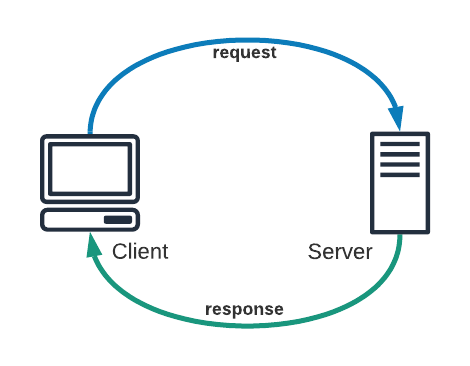
\includegraphics[width=\textwidth/2]{assets/Architectural-Design/Client-Server.png}
        \caption{Client-Server paradigm}
        \label{client_server_par}
    \end{center}
\end{figure}

As figure \ref{client_server_par} represents, the system is a distributed application which follows the common known client-server paradigm.

In particular, the client is \textit{thin}, which means that it does not contain the application business logic, but only the presentation layer. The server, instead, is \textit{fat} and contains all the data management and business logic.

In this section the architecture will be described in an easy way, justifying all the choices for adopted patterns.

\begin{figure}[H]
    \begin{center}
        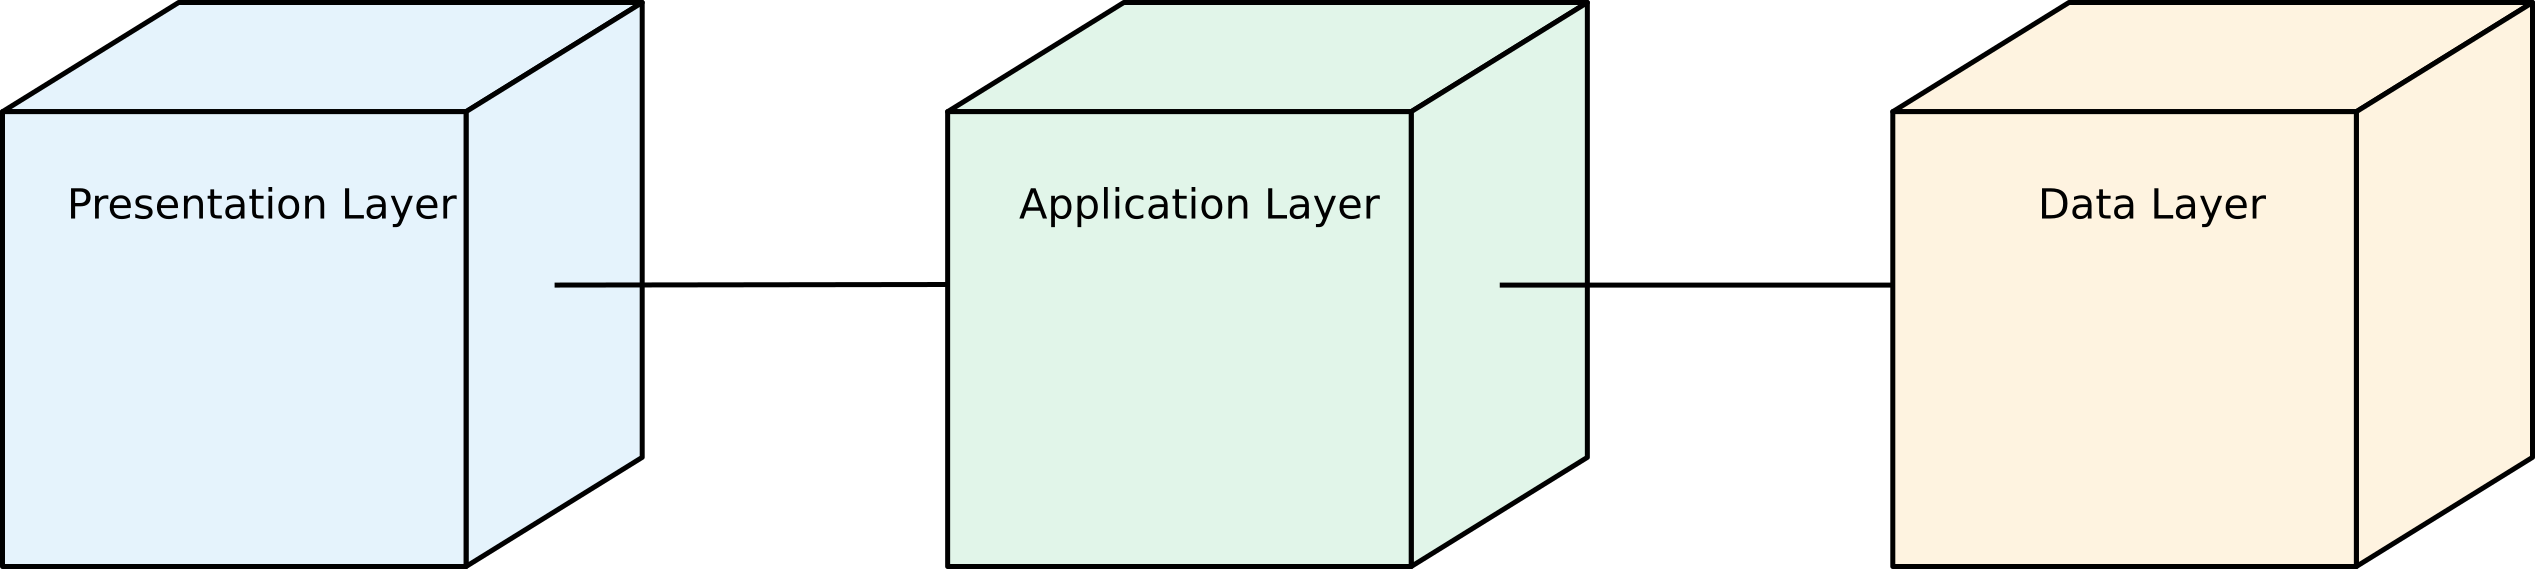
\includegraphics[width=\textwidth]{assets/Architectural-Design/3-tier.png}
        \caption{Three layers application}
        \label{three_tier_desc}
    \end{center}
\end{figure}

In figure \ref{three_tier_desc} the three S2B layers are shown, which respectively are:
\begin{itemize}
    \item \textbf{Presentation Layer:} it manages the presentation logic and, consequently, all the interactions with the end user. This is also called \textit{rendering layer}.
    \item \textbf{Application (Logic) Layer:} it manages the business functions that the S2B must provide.
    \item \textbf{Data Layer:} it manages the safe storage and the relative access to data.
\end{itemize}

As shown in the high level representation of figure \ref{three_tier_application} the S2B is divided into three layers that are physically separated by installing them on different tiers. A tier is a physical (or a set of) machine, each of them with its own computational power.

The application described in this document is composed by four tiers.

\begin{figure}[H]
    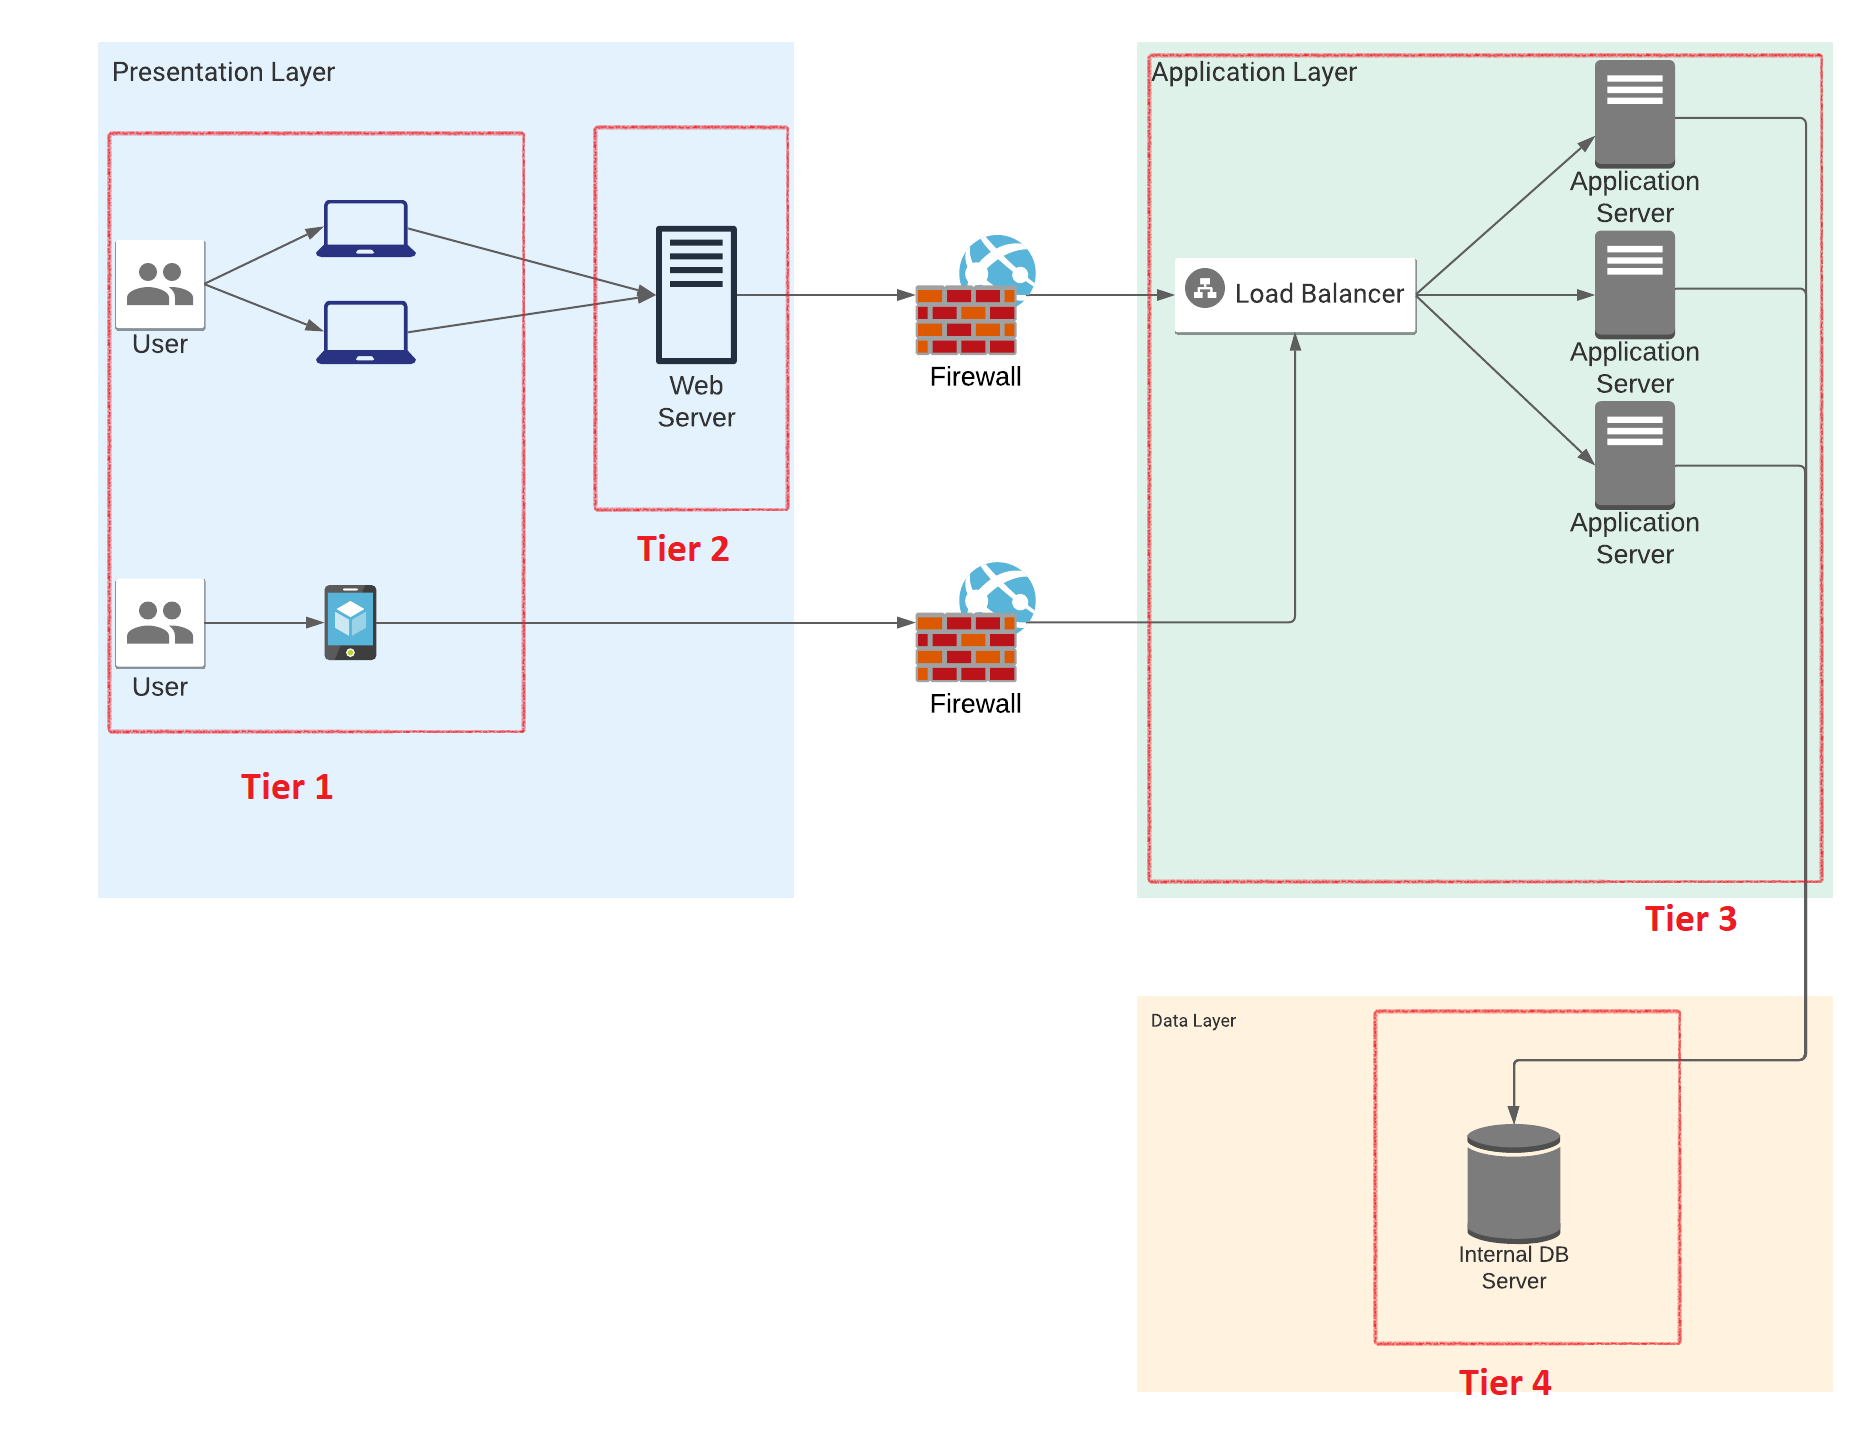
\includegraphics[width=\textwidth]{assets/Architectural-Design/ApplicationArchitecture.png}
    \caption{Architecture of the application}
    \label{three_tier_application}
\end{figure}

The service is supposed to be accessed through both a web interface and a mobile application, and this is valid for all kinds of users.

To make possible the construction of the web application, a client-side scripting paradigm will be adopted; this one will be described in detail in the final section of this document.

The architectural figure divides the application in the layers described above, and contains a Web Server, which act as a middleware between the user's browser and the application servers.
In case of using the mobile application, instead, the core of the software installed on user's device will interfaces with the business layer's APIs, which send and receive all the information in order to work properly directly to the application servers.

Finally, the application servers interfaces with the DBMS APIs, in order to retrieve and store the data required for the considered computation.

The nodes are separated by firewalls to guarantee a higher level of security of the whole system.

All the component will be described in depth in the following sections.

According to RASD specifications, if a buyer decides to purchase the third module option, which includes the installation on organization's servers, the entire architecture will be deployed and configured on that servers, without interfacing with CLup ones.

Otherwise, if the buyer intends to purchase only module 1 or module 2, the end user will interface with official CLup servers.

\subsection{Component View}

\begin{figure}[H]
    \begin{center}
        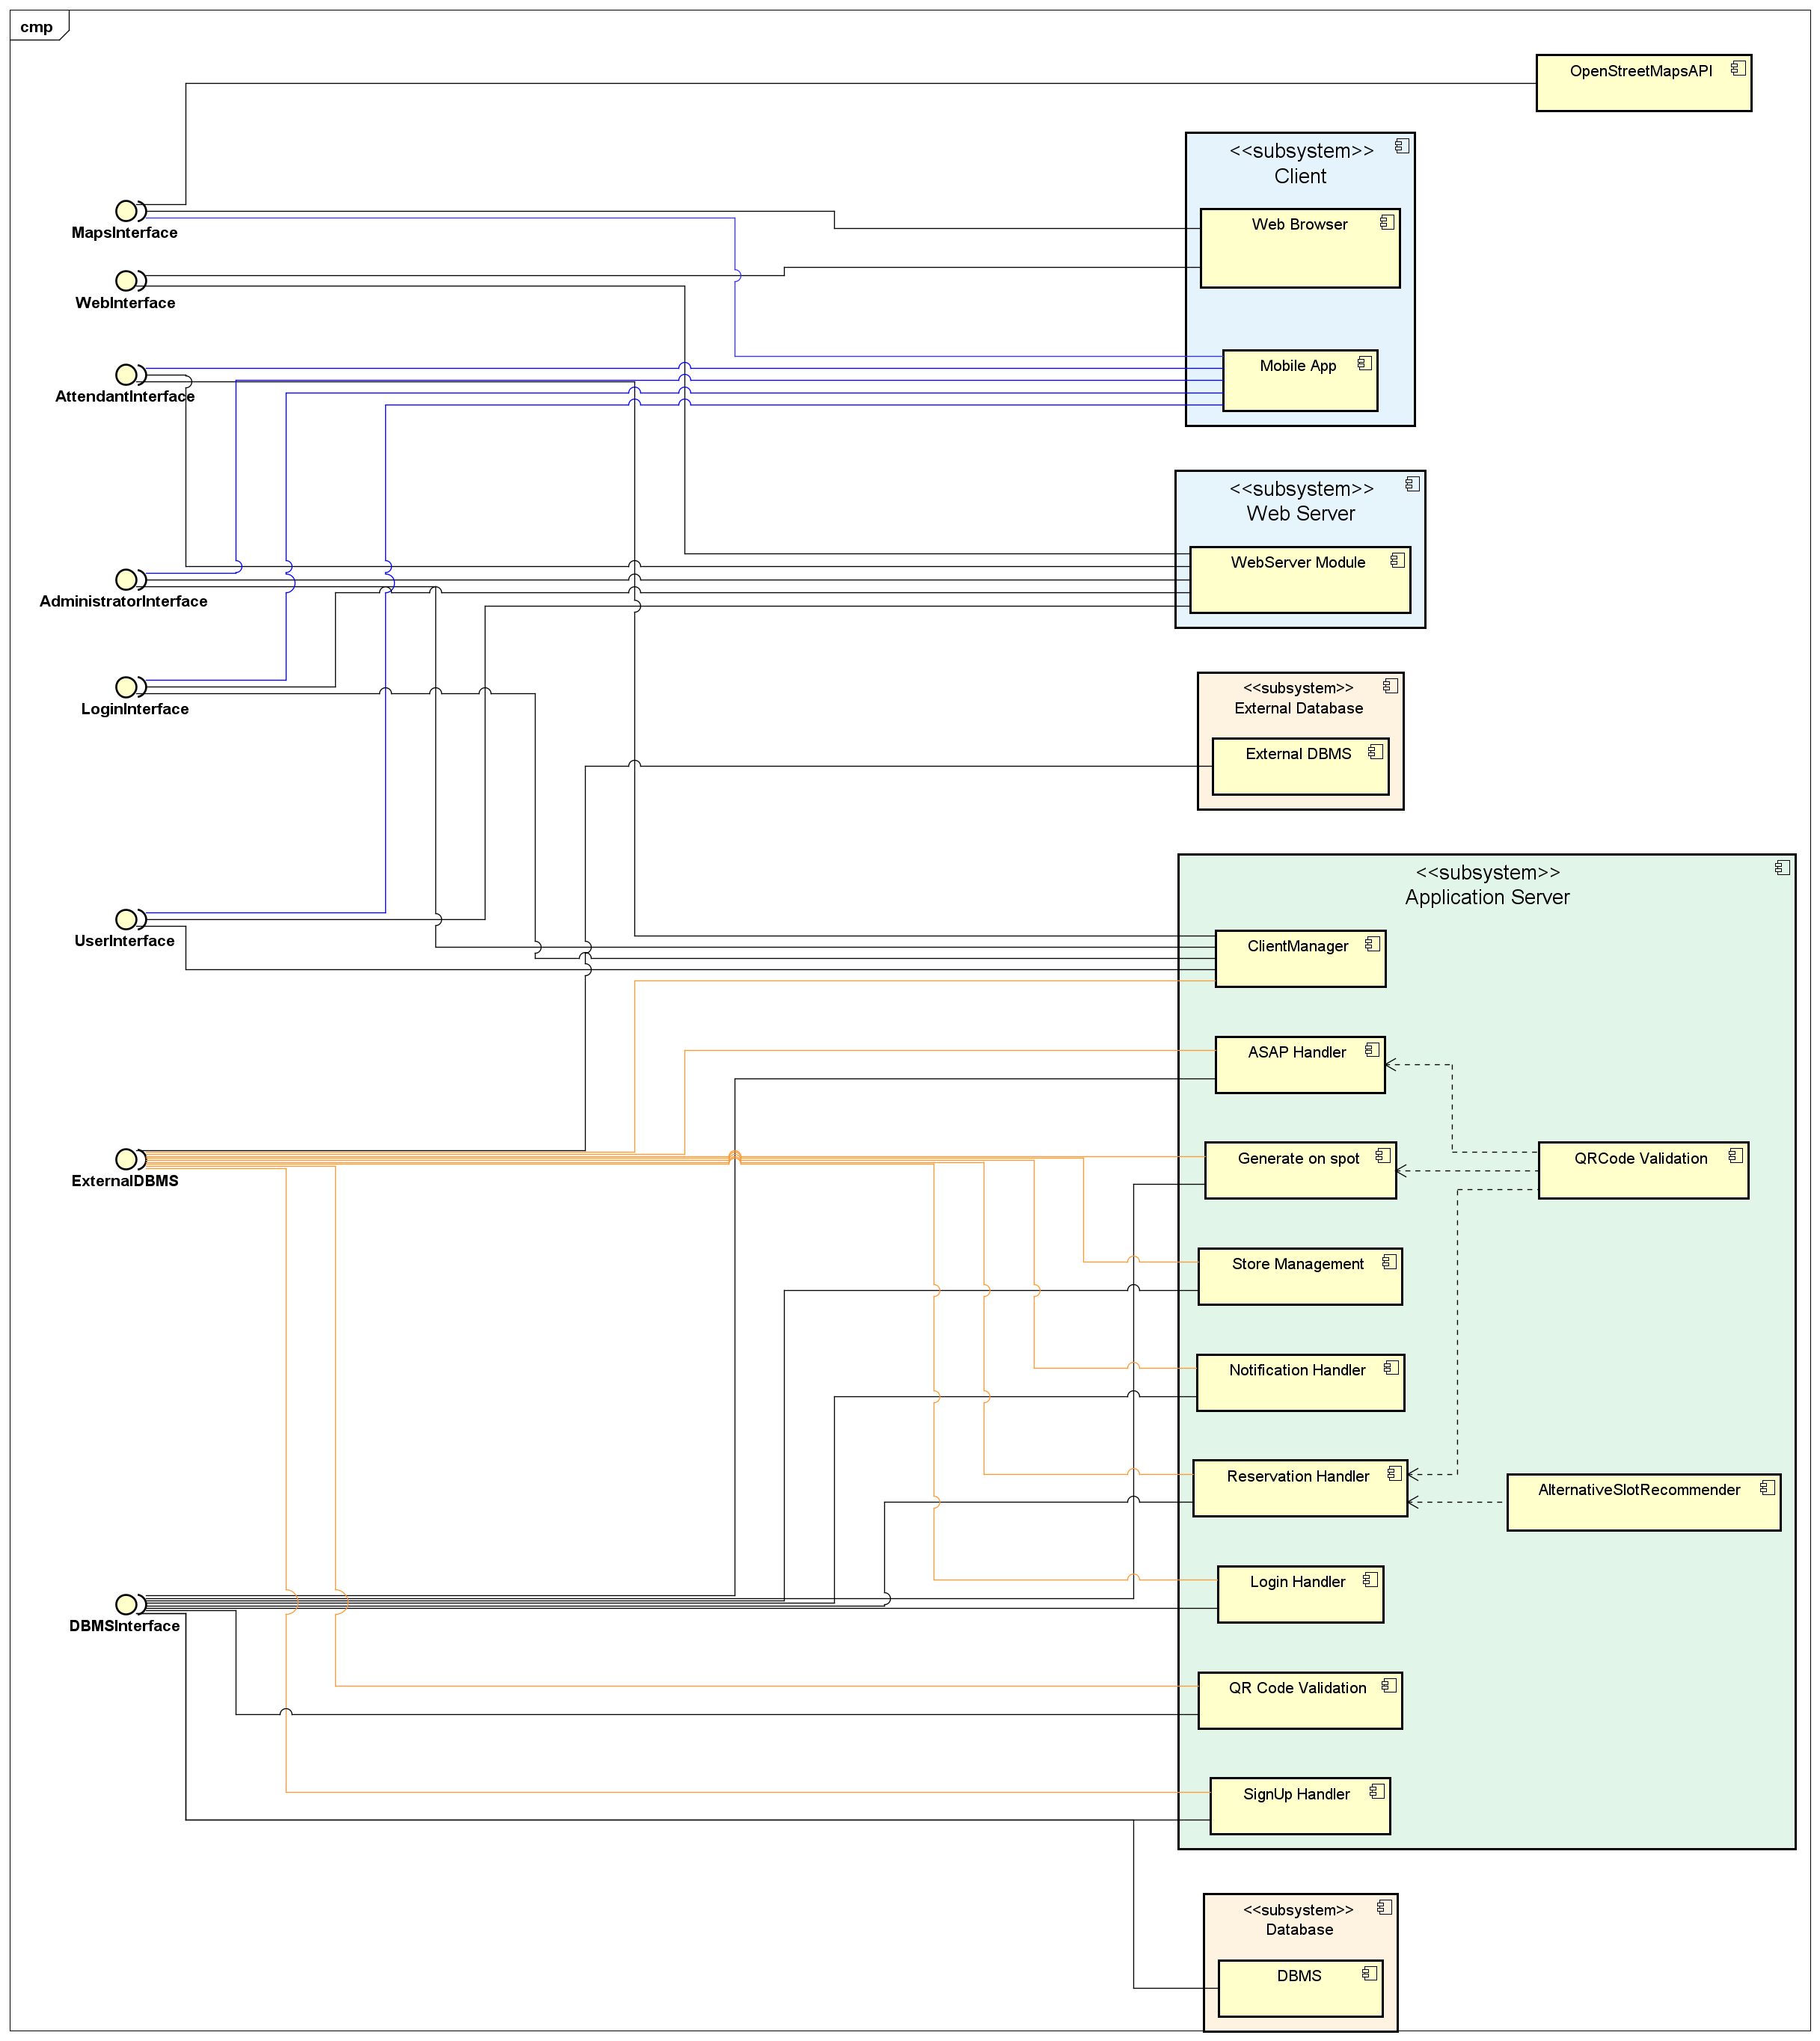
\includegraphics[width=\textwidth]{assets/Architectural-Design/ComponentDiagram.png}
        \caption{Component Diagram}
        \label{component_diagram}
    \end{center}
\end{figure}

In figure \ref{component_diagram} we can see a more detailed diagram representing the layers described before.

The web server has the function to route the browser requests to the application server and send back its responses.

\begin{itemize}
    \item \textbf{Client Manager}\\This module handles all the requests made by the client. At the beginning, while the client is not logged in, the module offers a \textit{loginInterface} which permits to execute a sign up or sign in operation. Once the client has logged in, the module shows only the other types of interfaces relying on user's role. A client logged as a user will exploit the \textit{UserInterface}, a store attendant an \textit{AttendantInterface} and a store administrator an \textit{Administrator Interface}.
    \item \textbf{Login Handler}\\This component handles the process of sign in. It receives the credentials inserted by the user (which are username and password) and checks for a correspondence in the database. If it found something, the user becomes authenticated and can continue to the correct private area.
    \item \textbf{SignUp Handler}\\This module's goal is to permit a user registration to the CLup service. There are three different sign up processes, each for every account type. The default registration flow, as the application's main target is a customer, provides the steps in order to register as user. However, at the beginning of the process, a prompt permits to switch sign up type to \textit{Attendant} or \textit{Administrator}. Some data will be asked to the registering client such as, in the main case, an email and a password.
    \item \textbf{ASAP Handler}\\This component handles the process of the MVP (see RASD section 1.1), which is the \textit{Retrieve a ticket} functionality. A registered and authenticated user selects the desired grocery store and requests, through a button, a new ticket. The S2B then provides an unique queue number, an estimated waiting time and a QRCode to check-in.
    \item \textbf{Reservation Handler}\\This is the second module of our S2B described in s. 1.1 of RASD document. Through this component, the registered and authenticated user can select a store and book a visit slot in the desired date and time (if available). The component can also optionally receive from user an estimated duration and a shopping list, in order to optimize people flows in the structure. Once the computation has finished, the component returns to user a confirmation, together with a QRCode to check-in.
    \item \textbf{Notification Handler}\\The goal of this component is to handle notifications of imminent calling of a ticket. In fact, when a number is going to be called, a trigger is generated, which sends an instant notification to the user who retrieved that ticket.
    \item \textbf{Generate on spot}\\This module handles the manual procedure of generating a ticket on the spot. In fact, when a user cannot sign up to CLup service, there is the possibility of going physically to the desired store and ask to be queued up. The attendant, through this component, sends a request of retrieving of a ticket, and the server returns the first slot available. This ticket is then printed, together with a QRCode generated from the system.
    \item \textbf{QRCode Validation}\\The functionality carried out from this component is the \textit{check-in} one. When a user arrives at the store, the attendant scans the QRCode generated from the application (or printed on the reservation) and lets the user entering the structure. The attendant scans the ticket (through CLup mobile app) with the integrated camera of a smartphone. The application then sends a request of check-in to the server, which responds with a status of the request (which can be either valid or invalid).
    \item \textbf{QRCode Generation}\\The goal of this module is to generate the QR Code of the ticket from a pre-defined string, which can be seen as the unique id of the ticket.
    \item \textbf{Alternative Slot Recommender}\\This component's aim is to suggest alternative slots to the end user, relying on people flows estimation from the other bookings.
    \item \textbf{Store Management}\\This last module handles the store administrator's personal area. In fact, it permits editing store information, which includes opening hours, maximum slots capacity, booking management and so on.
\end{itemize}

\subsection{Deployment View}

\begin{figure}[H]
    \begin{center}
        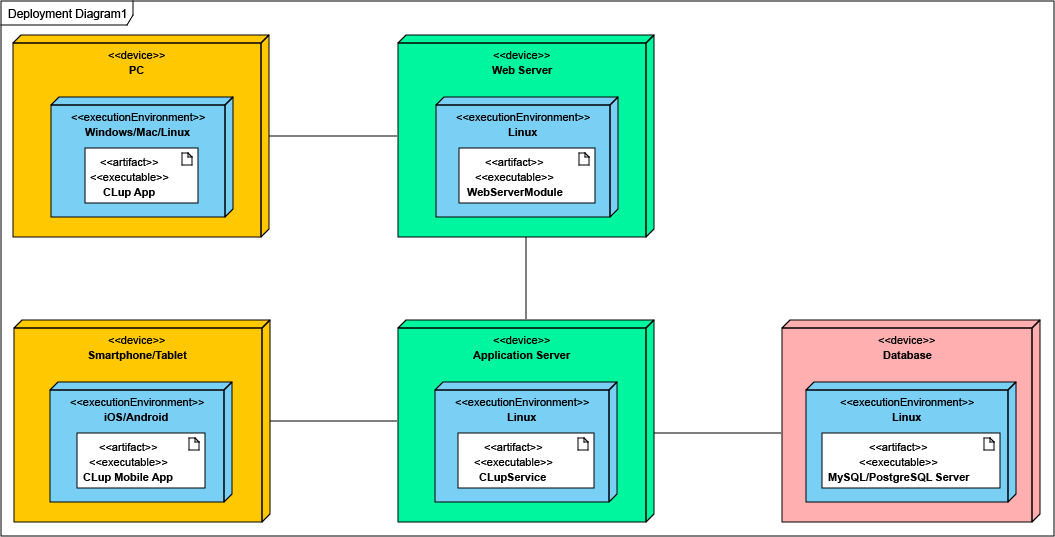
\includegraphics[width=\textwidth]{assets/DeploymentDiagram/DeploymentDiagram1.png}
        \caption{Deployment Diagram}
        \label{deployment_diagram}
    \end{center}
\end{figure}

The deployment diagram in figure \ref{deployment_diagram} shows the needed components for a correct system behavior, except the Maps APIs and the Authentication APIs ones.

Each device has its own Operative System where the software run. The tiers in the image are the following:
\begin{itemize}
    \item \textbf{Tier 1:} it is the client machine, which can be a computer with a web browser (running, for example, on Windows 10 OS) or the downloadable mobile application (available on both Apple's store and Google's Store).
    \item \textbf{Tier 2:} it is the web server, which does not execute any business logic, but it simply receives requests from the client, routes them to the server and wraps the application server's response into an HTML file, sending it back to the client. It also appends the styling logic of the page (CSS sheets, JS sheets, etc.).
    \item \textbf{Tier 3:} it is the application server, which runs the core functionalities of the S2B. The whole application layer is mapped into this tier, which communicates to the client tier through the web server and to the data tier through the DBMS gateway.
    \item \textbf{Tier 4:} it is composed by the database servers (DBMS, database). They store the data and execute actions on it, according to the instruction given by the application servers.
\end{itemize}

\subsection{Logical Description of Data}
\begin{figure}[H]
    \begin{center}
        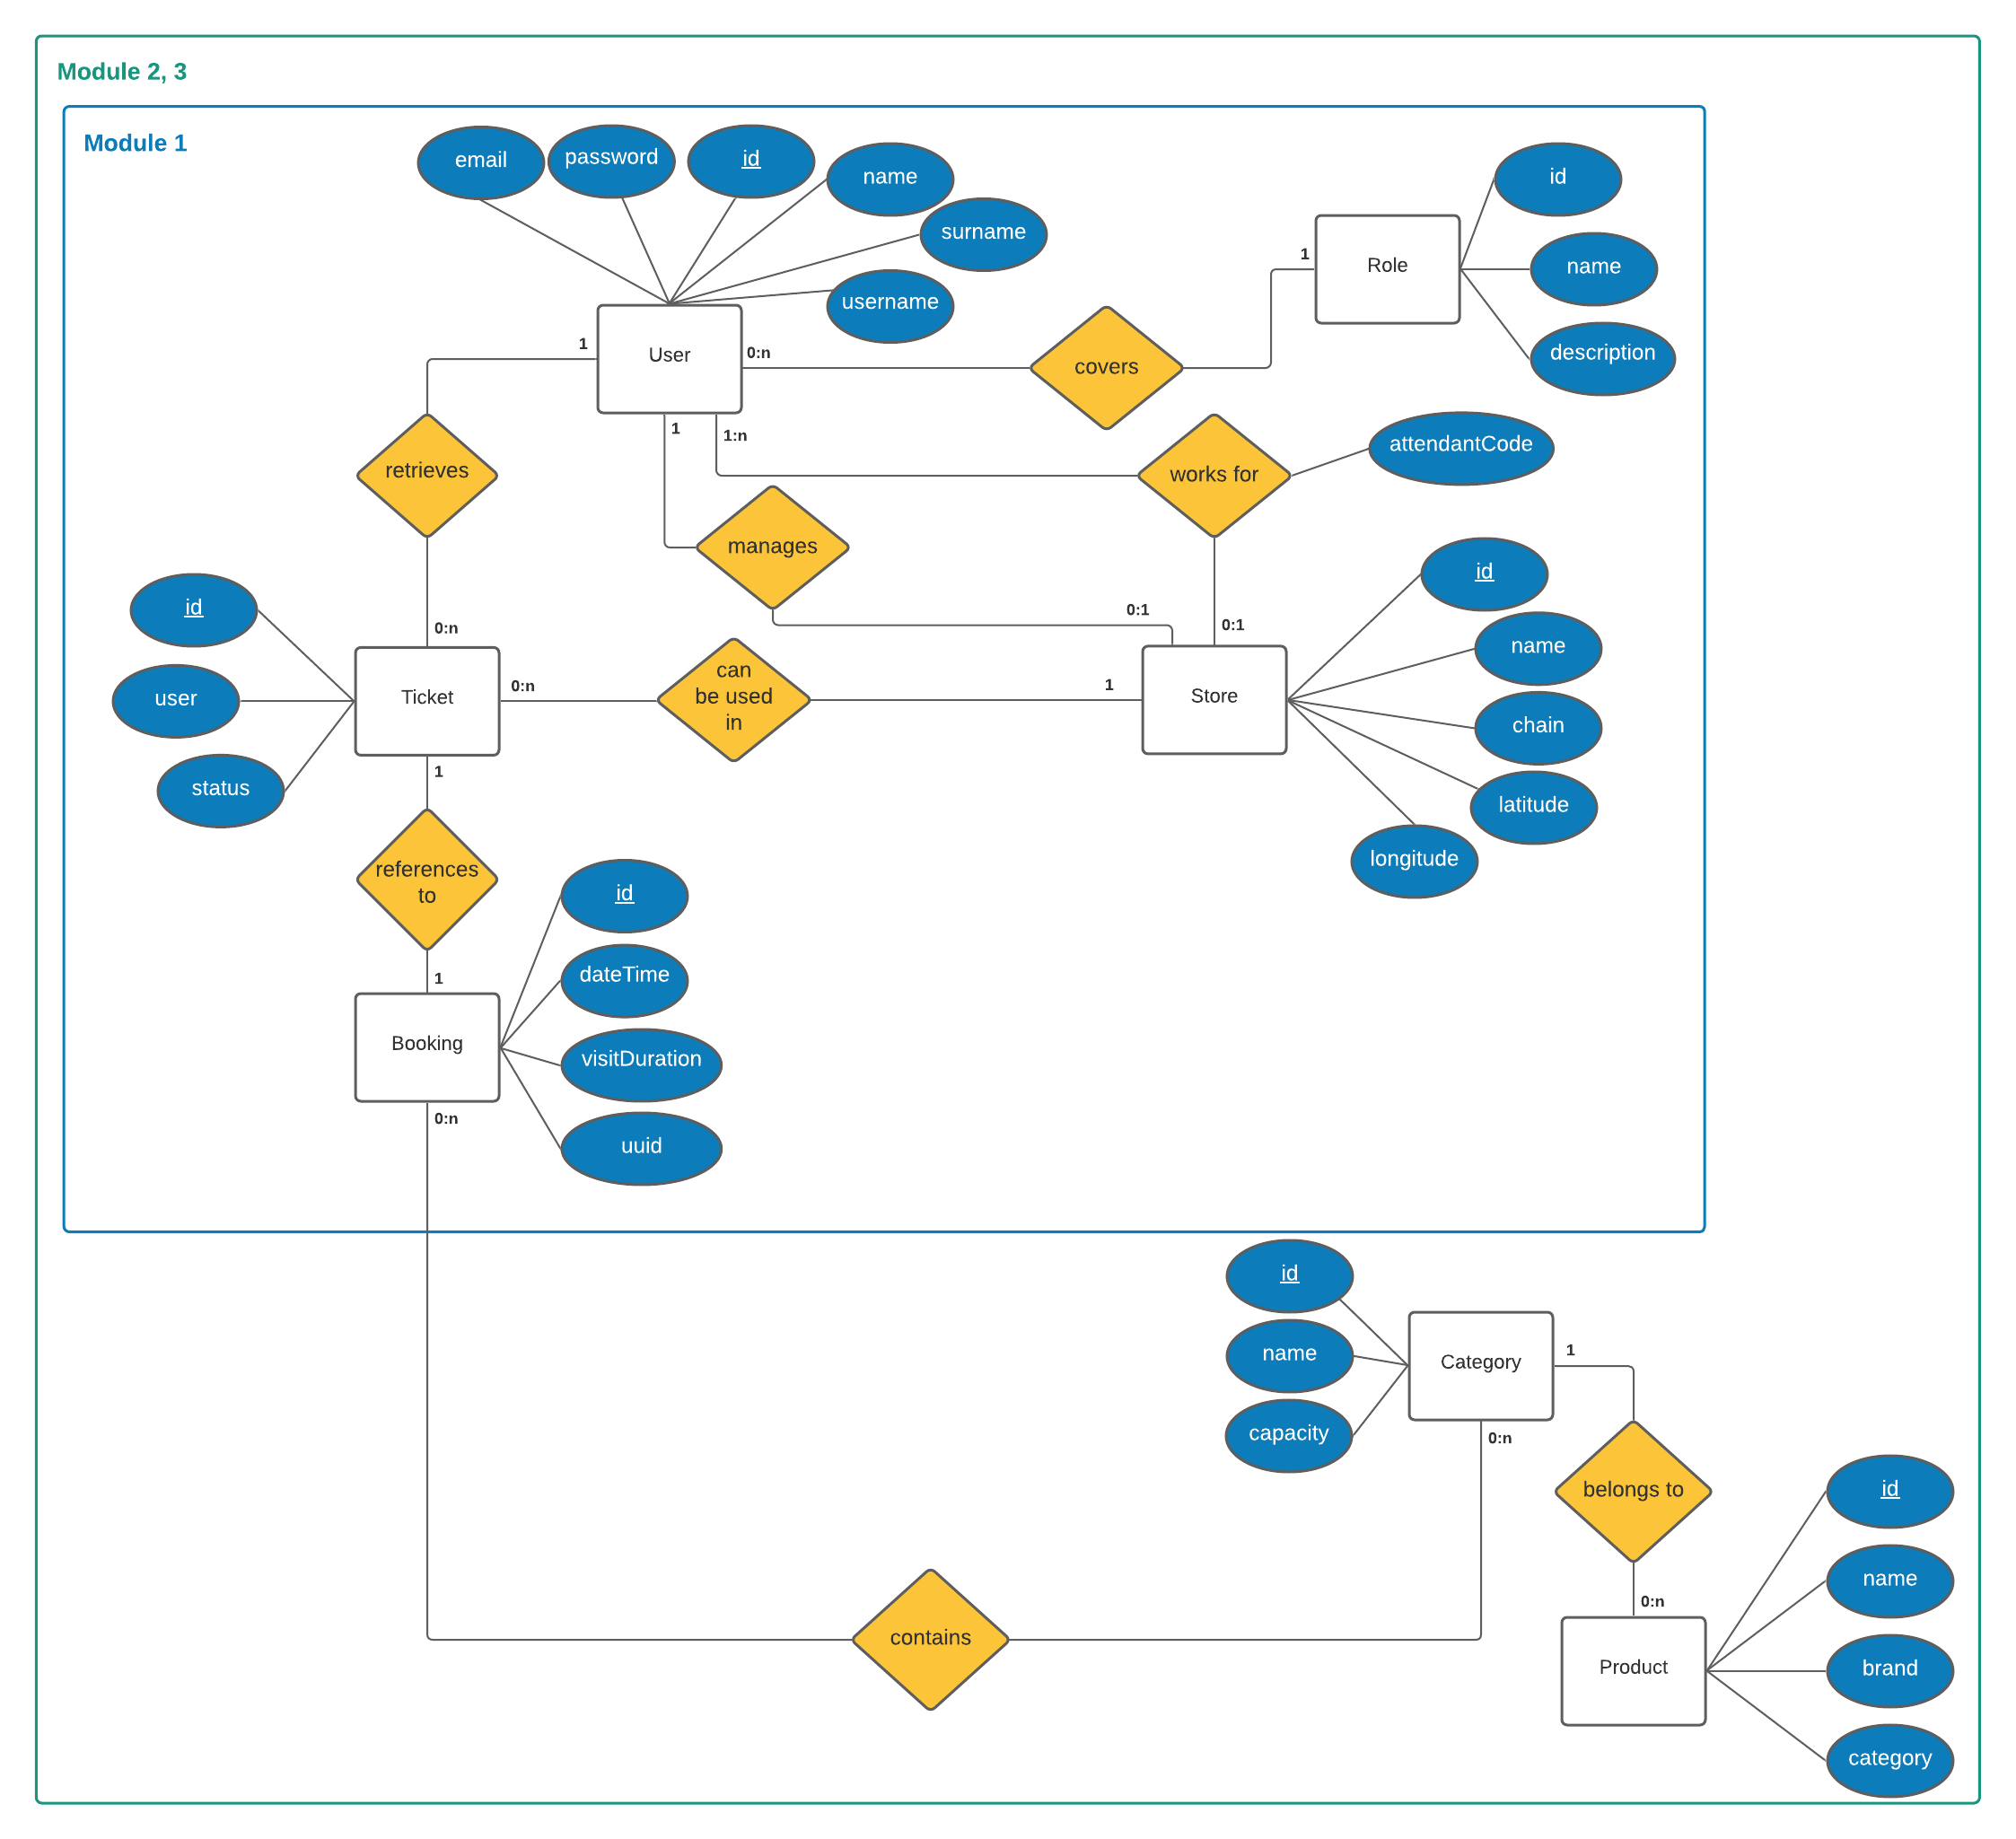
\includegraphics[width=\textwidth]{assets/Architectural-Design/ER.png}
        \caption{ER Diagram}
        \label{er_diagram}
    \end{center}
\end{figure}
The diagram in figure \ref{er_diagram} shows a logic representation of what kind of data is stored in the internal database of the S2B.

First of all, we can see the distinction in different modules (as s. 1.1 of RASD explains) and their respectively database structure in case of deployment on organization's servers. Of course, if the buyer chooses to remain on CLup official servers, the structure will remain the entire one, limiting the functionalities store by store.

The most important fact is that there are three different tables, each one for each customer type. In fact, since they contain different types of information, the most intuitive choice is the one of separating these types of data.

We then can see a table containing the list of all tickets, each of them associated to a specific store and (in case of \textit{Reservation} functionality) to a specific booking.

Finally, a booking can contain a list of categories, each one with a set of product inside it.

Looking at the relations, we can see that there is a \textit{bridge table} between Booking and Category, which associates a set of categories to one or more bookings. This association is used if a customer decides to insert a list of product in a reservation request.

\subsection{Architectural Style and Patterns}
\subsubsection{Four-tiered architecture}
The choice is on this architecture for many reasons:
\begin{itemize}
    \item \textbf{Flexibility:} \todo[]{Insert here}
    \item \textbf{Scalability:} an application divided on several tiers guarantee that the approach of scaling the architecture is adopted only for the most critical components. The result obtained maximizes the performance but also minimizes the costs.
    \item \textbf{Load Distribution:} the presence of several application server, preceded by a load balancer, guarantees that a single node would not become over-requested, sending the entire system down.
\end{itemize}

\subsubsection{RESTful Architecture}
The restful application will be adopted both on web and mobile side. This architecture is based on the stateless principle, in which the server does not contain any information about the state of client, that is managed directly on client side.

An useful property of this architecture is the \textit{code on demand} one, which permits sending some code snippets from the server to the client, and then make the client executing them locally (usually in the web browser). This behavior guarantees less computational load on the server and also a dynamic attitude of the service.

The application is then intended to be developed through \textit{client side scripting}, which means that all requests and update of the page are made on client side. This behavior also improves the user experience, and prevent refreshing the page each time an action is made.

\subsection{Other Design Decision}
\subsubsection{Scale-Out}
This method consists of cloning the nodes in which we expect to have a bottleneck in order to increase the general system scalability.

This choice leads to a higher deployment effort but also to a lower hardware upgrade cost when the limits are reached. In conclusion, the scale-out is a preferable road.

Once split, the system requires a load balancer in order to correctly redirects the incoming requests to the node with the lowest workload.

\subsubsection{Thin client and fat server}
This architecture consists of keeping as low information as possible on client side. It means that the business logic resides only on server side.

The minimum requirement of this choice is a stable connection between the parts; otherwise the application would not work as expected.

Of course, the main advantage of choosing this implementation style is that the client machine is not required to have an high computational power.

\section{User Interface Design}
The aim of this section is to show the design of the main screens of the User app, describing the flow of the main functionalities for which the application was intended. The flow is created according to specific and illustrated input of the final user \\
\textbf{Please note that} we used some mockups presented in the RASD but more mocks have been created and added to this part in order to better clarify the user experience. In addition, we chose to show only screenshot of the mobile application because in our opinion Users would interact mostly with it. We want to remember that the application will work also on web browsers, but the design and the interfaces of the web app will derive from these ones, and the accurate design choices of them are out of the aim of this project. \\

\section{Requirements Traceability}
This section will shown the traceability between requirements and modules described in component diagram.

\begin{itemize}
    \item \textbf{R1:} The system allows registered users to select the store where they want to shop
          \begin{itemize}
              \item \textbf{Login Handler}: this module allows registered users to select a store if they provide a correct combination of username and password.
              \item \textbf{ASAP Handler} \textit{or} \textbf{Reservation Handler:} this module allows to select a store either in case of ASAP functionality choice or Reservation functionality choice.
          \end{itemize}
    \item \textbf{R2:} The system allows users to retrieve a queue number
          \begin{itemize}
              \item \textbf{ASAP Handler}
              \item \textbf{Generate on spot:} this module allows people who are not registered to CLup service to be queued up manually by the store attendants.
          \end{itemize}
    \item \textbf{R3:} The system generates a QR Code associated to the ticket
          \begin{itemize}
              \item \textbf{QRCode Generator:} this component allows the QRCode to be generated from the ticket id.
          \end{itemize}
    \item \textbf{R4:} The system allows Store Administrators to add GPS Position and opening hours of the store
          \begin{itemize}
              \item \textbf{Store Management:} this module allows store administrator to edit all the information about their stores.
          \end{itemize}
    \item \textbf{R5:} The system allows Store Attendants to register with their attendant code
          \begin{itemize}
              \item \textbf{Sign Up:} this module allows the three types of users to register to the platform of CLup.
          \end{itemize}
    \item \textbf{R6:} The system allows users to select a day/time slot from the available ones
          \begin{itemize}
              \item \textbf{Reservation Handler}
          \end{itemize}
    \item \textbf{R7:} The system allows users to add a list of products (categories) to purchase and the duration time of the visit
    \item \textbf{R8:} The system computes a prediction of expected time duration of a customer's visit
          \begin{itemize}
              \item \textbf{}
          \end{itemize}
    \item \textbf{R9:} The system recommends alternative day/time slots or store/chains to a user
          \begin{itemize}
              \item \textbf{Alternative slot recommender:} this component lets the system suggests alternative visit slots relying on people flows parameters.
          \end{itemize}
    \item \textbf{R10:} The system takes note about the actual queue number
          \begin{itemize}
              \item \textbf{ASAP Handler} \textit{or} \textbf{Reservation Handler}
          \end{itemize}
    \item \textbf{R11:} The system notifies the user when its queue number is going to be called
          \begin{itemize}
              \item \textbf{Notification Handler:} this module triggers an action when a number is going to be called and informs the user through a notification.
          \end{itemize}
\end{itemize}

Also the system attributes are guaranteed by the design choices explained in this document; more precisely:
\begin{itemize}
    \item \textbf{Easy usability}: guaranteed through a very simple, minimal and intuitive user interface. Since the main target of the application is the customer-side, the experience is designed to be very simple. In fact, there are only a few buttons with clear and precise functionalities. The aim is to complete the \textit{ASAP} ticket retrieval in no more than five taps (or clicks).
    \item \textbf{Reliability and Availability}: accomplished through a replication of the running application in different clones, following the \textit{scale-out} method. The physical nodes of the system would then work in parallel, avoiding system downtimes due to a failure. In fact, when a clone breaks down, there are others in parallel which can supply the requested service, but with some performance issues. The scope is to obtain at least 97\% of availability for each tier (the total system would then have 97\% of availability).
    \item \textbf{Security}: guaranteed through an encrypted communication between client and server. If the client is connecting through the web interface, connection moves on HTTPS protocol. Otherwise, connection goes on TLS protocol.
    \item \textbf{Cross Platform}: firstly obtained through a development of a web interface, which can be accessed from any type of connected device. The mobile application, instead, will be available only for iOS and Android users.
    \item \textbf{Maintainability and Modularity:} the first is accomplished through the second, because the application will be divided in some small parts (called modules) which interacts each other to provide the requested service.
\end{itemize}

\section{Implementation, Integration and Test Plan}
The S2B will be divided as follows:
\begin{itemize}
    \item Client: it includes either web browser or mobile application;
    \item Web Server;
    \item Application Server;
    \item Internal Database;
    \item External services (such as OpenStreetMaps, IdP providers, etc).
\end{itemize}

These elements will be implemented following a bottom up logic, in order to avoid stub structures that would be more difficult to implement and test.

The main focus is on the module of the application server, because of its importance in the S2B development and also due to its testing difficulty.

The following table presents the functionalities described in the RASD document and highlight for each of them the importance for the customer and the difficulty of their implementation.

\begin{center}
    \begin{tabular}{ | c | c | c |}
        \hline
        \textbf{Functionality}        & \textbf{Importance for customer} & \textbf{Difficulty} \\ \hline
        Sign Up and Login             & Low                              & Low                 \\ \hline
        ASAP (MVP)                    & High                             & Medium              \\\hline
        Make a reservation (module 2) & Medium                           & High                \\\hline
        Hand out on spot              & High                             & Medium              \\\hline
        Periodic notifications        & Low                              & High                \\
        \hline
    \end{tabular}
\end{center}

\todo[]{Descrivere l'implementazione di ciascun componente}

\subsection{Clarification on component integration}
\begin{center}
    \begin{figure}[H]
        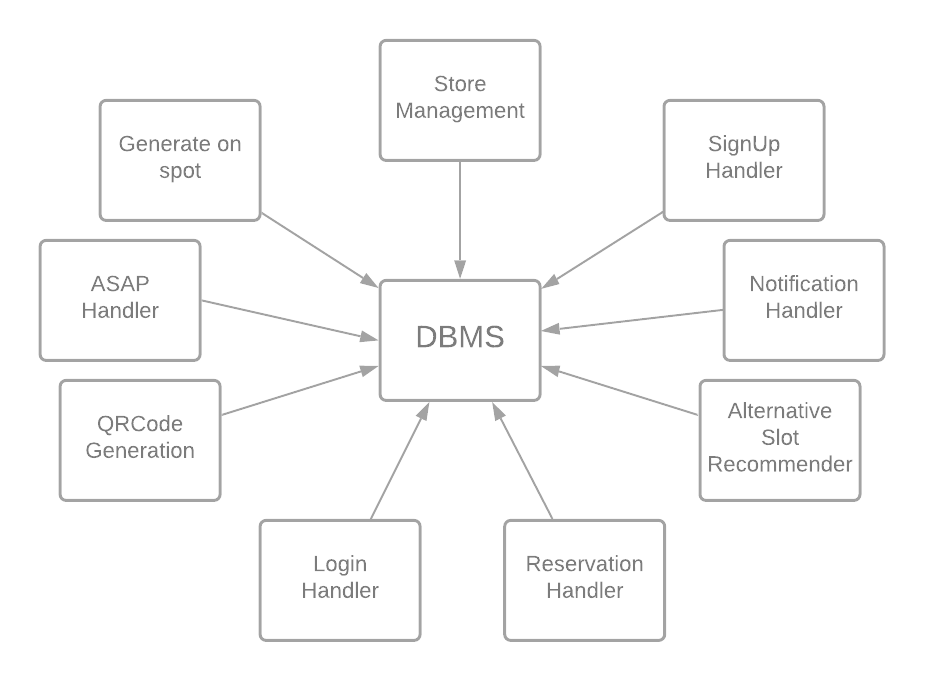
\includegraphics[width=\textwidth]{assets/ITPlan/Components-Integration.png}
        \caption{Components Integration}
        \label{components_integration}
    \end{figure}
\end{center}

\pagestyle{plain}

\section{Effort spent}
\begin{tabular}{ | c || c | c | c | c| c|}
    \hline
    Student        & Time for S.1 & S.2 & Time for S.3 & Time for S.4 & Time for S.5 \\ \hline
    Alice Piemonti &              &     &              &              &              \\ \hline
    Luca Pirovano  & 2h           & 7h  &              & 2h           &              \\ \hline
    Nicolò Sonnino &              & 3h  &              &              &              \\
    \hline
\end{tabular}

\end{document}
